\documentclass[Times,12pt,oneside,openany,print,index]{report}
\usepackage[a4paper,width=150mm,top=25mm,bottom=25mm]{geometry}
\usepackage[spanish]{babel}
\usepackage[utf8]{inputenc}
\usepackage{csquotes}
\usepackage{amsmath}
\pagestyle{plain}

\usepackage{graphicx}
\graphicspath{{./images/}}
\usepackage{caption}
\usepackage{array}

\usepackage[nottoc]{tocbibind}

\usepackage[normalem]{ulem}

\usepackage{hyperref}
\hypersetup{
    colorlinks=true,
    linkcolor=black,
    filecolor=magenta,      
    urlcolor=black,
    citecolor=black,
}
\urlstyle{same}

\usepackage{microtype}

\setlength{\parindent}{0em}

\usepackage[backend=biber,style=authoryear,sorting=ynt]{biblatex}
\addbibresource{bibliography/references.bib}

\let\cleardoublepage=\clearpage

\usepackage{etoolbox}
\AtBeginEnvironment{quote}{\small}
\captionsetup[figure]{font=footnotesize}

\begin{document}

\thispagestyle{empty}
\begin{titlepage}
\renewcommand*{\thepage}{Title}

    \begin{center} 
        \vspace*{3cm}
        
        {\fontsize{16pt}{22pt}\selectfont\textbf
            {Significación social y supervivencia simbólica en la producción de imagen artística sobre la resistencia y crisis del Hospital San Juan de Dios, Bogotá, 2000-2015}
        }


        
        \vspace{1.5cm}
        
        \text{Por:}
        
        \vspace{0.5cm}
        
        	JUAN CARLOS ARROYO SOSA, B.A. \\

        \vspace{1.5cm}
        
        	Tesis presentada a la Facultad de Artes y Humanidades \\
            de la Universidad de Caldas, en cumplimiento parcial de los requisitos \\
            para el grado de Magister en Diseño y Creación Interactiva

        
        \vspace{2.5cm}
        
        Asesora de Tesis:\\

        \vspace{0.5cm}
        
        BEATRIZ DEL CARMEN PERALTA DUQUE, Phd.\\
        
        \vspace{3cm}
        
            Universidad de Caldas\\
            \vspace{0.5cm}
            Artistic-2.0 license 2024. 
    
    \end{center}

\end{titlepage}
\cleardoublepage

\pagenumbering{roman}

\phantomsection
\addcontentsline{toc}{chapter}{Declaración de ética}
\section*{Declaración de ética}
\setlength{\parskip}{1em}

Yo, quién escribe este texto, he sido durante años un silencioso observador de el caso del San Juan, y como afectado contiguo al drama social derivado de la crisis y fin de los servicios hospitalarios, he visto los síntomas de decadencia funcional, deterioro de las edificaciones, y el drama humano vivido por las personas alrededor de la persistencia en las distintas formas de resistir al fin del HJSD. Una de esas trabajadoras a las que aún se les adeuda su liquidación, es mi madre, la enfermera Berenice Sosa o como aún después de tantos años de no ejercer su profesión, sus compañeras del San Juan le siguen diciendo “jefe Berenice”.

Esta investigación titulada \textit{Significación social y supervivencia simbólica en la producción de imagen artística sobre la resistencia y crisis del Hospital San Juan de Dios, Bogotá, 2000-2015} se ha realizado respetando los principios éticos fundamentales de integridad, transparencia y respeto hacia las personas y los materiales involucrados.  

La recolección de datos incluyó el uso de material de registro de obra artística, consulta bibliográfica, así como registro fotográfico personal y cedido temporalmente para consulta por ex trabajadores del hospital, quienes colaboraron de manera voluntaria y con su consentimiento informado. Se garantizó la confidencialidad de los participantes y el uso adecuado de los recursos proporcionados, asegurando que sus contribuciones fueran tratadas con el mayor respeto y se emplearan exclusivamente con fines académicos y de investigación.  

El estudio busca promover la comprensión de las dimensiones simbólicas y sociales de la resistencia y crisis del Hospital San Juan de Dios, contribuyendo a preservar su memoria histórica. Se evitó cualquier manipulación de la información recopilada y se actuó con responsabilidad frente a los derechos de los artistas, autores y participantes involucrados en este proceso.  

Esta tesis se adhiere a los principios éticos de la investigación académica y se compromete a actuar en beneficio de la verdad, el conocimiento y el reconocimiento cultural. 
\pagebreak

\phantomsection
\addcontentsline{toc}{chapter}{Resúmen}
\section*{Resumen}
\setlength{\parskip}{1em}

Esta investigación aborda los desafíos de las trayectorias convertidas en imagen relacionadas con los derechos laborales del arquetipo de enfermera del Hospital San Juan de Dios (HSJD), enfocándose en la experiencia personal de mi madre durante la crisis del hospital como \textit{wicked problem}. La pregunta central que guía este estudio es: ¿Cómo la imagen artística sobre la crisis y resistencia del HSJD entre 2000 y 2015 contribuye a la significación y supervivencia simbólica de este evento en la memoria colectiva?.

De acuerdo con las referencias bibliográficas y audiovisuales consultadas, la belleza estética del hospital, el atractivo de la ruina y la complejidad histórica han generado múltiples perspectivas de creadores visuales, artistas, periodistas e investigadoras académicas que han observado y documentado el HSJD. \textcolor{edit30sept}{Sin embargo, esta prolífica producción no ha logrado generar para las enfermeras satisfacción en términos de justicia laboral y simbólica. La situación se presenta como un entramado complejo, lleno de expectativas fallidas, en el que al menos 3.640 personas quedaron desempleadas y aproximadamente 1.500 trabajadores no recibieron su liquidación.}

La investigación se desarrolla como una meta-composición estética y documental que trasciende la mera documentación o el análisis sociopolítico. Se sustenta en los campos de la antropología de la imagen, estudios visuales y sociosemióticos, para crear un fundamento argumentativo que permita «trabajar» con imágenes, que es, en esencia, pensar a través de las imágenes.

Metodológicamente, se operacionaliza el análisis mediante la apropiación de la idea de montaje, complementada con la identificación de imaginarios sociales y estructuras semióticas denominadas imágenes-síntoma y anacronismos. Esta aproximación permite interpretar cómo diversas acciones simbólicas, argumentales y estéticas evidencian una intensa producción visual en torno a la crisis del HSJD.

Los resultados revelan que los registros de estas acciones conforman un \textcolor{edit30sept}{ \emph{corpus}} de imágenes que permite interpretar tanto los síntomas visuales de la crisis sistémica como el deterioro arquitectónico y patrimonial en su interacción con el drama humano y social. La investigación demuestra cómo las representaciones visuales del HSJD trascienden la mera documentación para convertirse en evidencias del drama humano y la defensa de un bien público. \textcolor{edit30sept}{La tesis expone, mediante la metodología del montaje y la meta-composición estética y documental, la disrupción del fenómeno del San Juan, mostrando cómo estas operaciones visuales ofrecen oportunidades de reconfiguración de sentido en la memoria colectiva.}

Este estudio contribuye al campo del diseño y creación interactiva al proponer una metodología específica para el análisis de memoria social a través de la imagen, donde el montaje artístico se integra como medio de exploración y validación de hipótesis sobre la supervivencia simbólica de eventos críticos en el imaginario colectivo.

\vspace{1cm}
\textbf{Palabras clave:} \textcolor{edit30sept}{Meta-composición estética, montaje visual, imagen-síntoma, interfaz de memoria, crisis hospitalaria, Hospital San Juan de Dios Bogotá.}
\pagebreak


\phantomsection
\addcontentsline{toc}{chapter}{Dedicatoria}
\section*{Dedicatoria}

\vspace{2cm}

A todas las personas (vivas o muertas, locas o cuerdas) que han luchado por sus derechos laborales y el espíritu del cuidado humano en el Hospital San Juan de Dios de Bogotá.

\vspace{4cm}

\subsection*{Agradecimientos}
A mi esposa, quien me ha acompañado con amor y paciencia en este proceso; a mi madre, cuyo ejemplo de lucha y resistencia ha sido una inspiración constante; a mis profesores y tutores; y a todas las personas que, de una forma u otra, contribuyeron a la realización de este trabajo. Su apoyo ha sido un pilar fundamental a lo largo de este viaje, especialmente en los momentos en que las dificultades de la vida hicieron que observar y escribir se convirtieran en un refugio y una fuente de alivio.
\pagebreak

\phantomsection
\addcontentsline{toc}{chapter}{Licencia}
\section*{Artistic License 2.0}

El autor ha decidido licenciar esta obra bajo los términos de la Artistic License 2.0, permitiendo que cualquier persona:
\begin{itemize}
    \item Copie, modifique y distribuya el trabajo original o modificado.
    \item Cree versiones derivadas de la obra, siempre y cuando se indique claramente que se realizaron modificaciones.
\end{itemize}

\subsection*{Términos de la Licencia}

Al usar esta obra, aceptas que:

\begin{itemize}
    \item Debes incluir un aviso claro que indique si el trabajo ha sido modificado y qué cambios se han realizado.
    \item No puedes utilizar el nombre del autor original para promocionar productos derivados sin permiso explícito.
    \item El código fuente o el material base debe estar accesible para cualquier versión distribuida.
\end{itemize}

Para más información sobre la licencia, consulta el texto completo en inglés en el siguiente enlace: \href{https://opensource.org/licenses/Artistic-2.0}{Artistic License 2.0}.

---

\subsection*{Aclaración sobre fotografías y registros de obras}

Las imágenes de registro de obras de otros creadores y las fotografías incluidas en esta tesis, en particular aquellas compartidas por las extrabajadoras del Hospital San Juan de Dios (HSJD) y referidas en el texto, \underline{son de autoría y licencia de sus propios autores}.

Estas imágenes no comparten la licencia Artistic License 2.0 del texto de la tesis. Su uso y distribución están sujetos a los derechos de autor y licencias aplicables según lo determinado por sus respectivos autores.

Se recomienda contactar directamente a los autores o titulares de los derechos de las imágenes si se desea obtener más información sobre sus condiciones de uso.


\listoffigures
\listoftables   

\renewcommand{\contentsname}{Tabla de contenidos}
\cleardoublepage
\phantomsection
\addcontentsline{toc}{chapter}{Tabla de contenidos}
\tableofcontents

\pagenumbering{arabic}

\chapter{Conceptualización del problema}
\section*{Introducción al fenómeno}

La crisis del HSJD emerge como un laboratorio social donde el diseño y la creación interactiva pueden explorar las dinámicas de transformación institucional, memoria colectiva y resistencia ciudadana. Más allá de una indagación entre registros documentales o artísticos, este estudio pretende señalar cómo diversas acciones simbólicas, argumentales, documentales y estéticas evidencias de una intensa atracción visual en torno a la crisis del HSJD, los registros de estas acciones nos brindan un corpus de imágenes con potencial para interpretar los síntomas visuales de la crisis sistémica, así como los deterioros arquitectónicos y patrimonials en juego con el drama humano y social.

El caso del Hospital San Juan es emblemático dentro del contexto de las crisis sociales e institucionales generadas por los cambios masivos en los sistemas de salud orientados al servicio público. ¿Cómo comprender, explicar e interpretar los registros visuales y las obras que serán tratadas como \guillemotleft evidencias\guillemotright\ que articulan el drama humano y la defensa de un bien público?. 

A estas evidencias las denominamos imagen-síntoma, una presencia disruptiva en la imagen que interrumpe el curso normal de la representación: supervivencias, latencias y reapariciones que habitan las imágenes. La metodología aplicada a la colección visual de memoria social permite abordar el fenómeno a través de la imagen.

El concepto de imagen-síntoma\footnote{\begin{quote}La idea de la imagen como síntoma es lo que quiere tomar Didi-Huberman de Freud y aplicarlo al campo de la historia del arte. Por supuesto, no sobra decir que se trata de dos disciplinas muy distintas, que la experiencia de las imágenes oníricas no es igual a la de las imágenes artísticas. Aun así, el uso del carácter sintomático de la imagen en la historia del arte no es tan diferente al del análisis de los sueños. Sólo que aquí, en lugar de evocar lo onírico, Didi-Huberman lo utilizará para nombrar esa perturbación que lo visual causa dentro de lo visible. \parencite[p. 37]{VegaArevalo2017}\end{quote}} resulta fundamental para comprender cómo las representaciones visuales del HSJD trascienden la mera documentación para convertirse en manifestaciones de tensiones sociales más profundas. Según Didi-Huberman, estas imágenes actúan como síntomas que revelan conflictos latentes en el tejido social.

\begin{quote}
Si la imagen es un síntoma -en el sentido crítico y no clínico del término-, si la imagen es un malestar en la representación, es porque indica un futuro de la representación, un futuro que no sabemos aún leer, ni, incluso, describir. \parencite[p. 177]{DidiHuberman2011}
\end{quote}

Este estudio indaga en el papel fundamental de la imagen para la contemplación profunda de los fenómenos sociales, ofreciendo nuevas perspectivas para comprender su complejidad y contribuyendo al debate sobre el papel del arte y el diseño en los procesos de cambio social y la construcción de memoria colectiva.

El diseño, entendido como práctica crítica y performativa, permite desvelar las capas de significado ocultas en los registros visuales. No se trata solo de documentar, sino de construir narrativas que revelen las tensiones sociales subyacentes. Las imágenes del HSJD se convierten así en interfaces de memoria, donde cada fragmento, cada ruina, cada registro artístico funciona como un nodo de información compleja.

La creación interactiva se presenta como sugerencia para trascender la observación pasiva, invitando a una participación activa en la construcción de sentido. En este contexto, las obras artísticas y los registros visuales no son meros documentos, sino dispositivos de activación memorial que permiten:

\begin{itemize}
    \item Desarticular narrativas oficiales sobre el abandono institucional
    \item Visibilizar las experiencias de los trabajadores y comunidades afectadas
    \item Generar nuevas formas de comprensión y elaboración del conflicto social
\end{itemize}

\section*{Contextualización histórica}

El Hospital San Juan de Dios de Bogotá fue fundado en 1723 como un centro de atención médica y asistencia social para los más necesitados. A lo largo de los siglos, el hospital se convirtió en un referente de la salud pública en Colombia, atendiendo a miles de pacientes y formando a generaciones de profesionales de la salud. Sin embargo, a partir de la década de 1990, el HSJD comenzó a experimentar una serie de crisis institucionales y financieras que llevaron a su cierre.

En el año 2001, coincidiendo con la salida del último paciente, “3.640 personas quedaron desempleadas, y aproximadamente 1.500 trabajadores no recibieron la liquidación correspondiente por sus años de servicio” \parencite{Castiblanco2017}. No obstante, este hecho fue solo uno de los múltiples detonantes de las acciones de resistencia que se han desarrollado a lo largo de los años en torno a este caso. Los afectados directos emprendieron diversas formas de lucha y resistencia frente a la pérdida de sus empleos y de un espacio vital para su realización personal y profesional. Estas, sin embargo, no fueron las únicas motivaciones ni las únicas comunidades que centraron su atención en el complejo entramado sistémico de problemáticas sociales asociado al caso.

Ese hospital ya estaba en estado de malestar mucho antes de la salida del último paciente. De acuerdo con el profesor Mario Hernández investigador en historia de la medicina, en las décadas de los 70 y 80 inició la crisis de los Estados de Bienestar, que derivaron en acciones institucionales del pensamiento llamado neoliberal. Así, la dinámica económica global de tratar de buscar que los servicios de interés público como la salud fueran parte de las dinámicas de mercado condujeron al San Juan hacia un proceso de transformación. El Hospital que nació como beneficencia trató fallidamente de adaptarse a las nuevas demandas neoliberales, en consecuencia dejó de disponer tiempo o dinero para cuidar el patrimonio arquitectónico. El hospital se estaba descascarando mucho antes del embate de la Ley 100 y aún así se mantendría vivo y funcional hasta su último aliendo, cumpliendo su propósito de atención y cuidado de la salud.

Paralelamente a los esfuerzos institucionales para reabrir el San Juan, surgieron experiencias de lucha social, señalamientos estéticos y acciones memoriales que abordaron la complejidad del fenómeno. Esta investigación explora cómo se construye sentido a través del registro de obras e imágenes artísticas, estéticas, poéticas y no funcionales.

Fortalecer la conexión entre la contextualización histórica y el enfoque en las prácticas estéticas permite comprender cómo las imágenes del HSJD revelan tensiones sociales subyacentes y generan nuevas formas de comprensión y elaboración del conflicto social.

\subsubsection{Laboratorio social}

\subsubsection{Exhibición y creación}

\subsubsection{El San Juan clausurado}



\section*{Planteamiento del problema }
¿Ante el abandono qué hacemos? ¿nos quedamos, nos vamos, luchamos, por qué, …hasta cuando? En el año 2001 salió el último paciente del HSJD, un hito, sin embargo, ese día no se inhabilitó el San Juan. El abandono ya había comenzado años antes. Las gestiones institucionales para su liquidación y reapertura total han durado décadas, y a la fecha no es posible afirmar que el San Juan haya cerrado o abierto definitivamente.

Se presenta una contextualización espacial e histórica para darle sentido a la revisión de los signos de las resistencias, registros gráficos y audiovisuales de los procesos de creación artística, instalaciones in-situ, performativas y de dramaturgia, que, como veremos en el desarrollo de este informe, contienen signos icónicos e indicios de la imaginación social. En el año 2007 aparece una de las primeras manifestaciones artísticas que señalan explícitamente la problemática del HSJD, de allí en adelante y hasta el año 2016 serán producidas y exhibidas una docena de obras artísticas hechas en torno a esta situación.

Las imágenes analizadas a la luz del concepto imagen-síntoma tienen una carga de resistencia al olvido, no en si mismas, sino en aquello que cargan o permiten, son imágenes con las cuales es posible vislumbrar ruinas que son síntomas del drama humano y social, en el corpus de imágenes analizadas se evidencian recurrencias en el discurso desde distintos ámbitos de participación en el señalamiento a la crisis del San Juan. Las imágenes de registro, y respuestas críticas frente a una situación o evento de crisis nos exigen más de lo que explican, en ellas devienen explicaciones en aparente discordia.


\section*{Justificación y relevancia}
La crisis del Hospital San Juan de Dios HSJD representa una problemática sistémica donde convergen múltiples dimensiones interconectadas e interdependientes: económicas, administrativas, sociales, políticas y culturales. Desde la perspectiva del diseño y la creación interactiva, resulta pertinente abordar estas problemáticas sociales complejas con enfoques y metodologìas innovadoras, especialmente en el actual contexto colombiano de construcción de paz, donde la transformación social requiere trascender la resolución del conflicto armado para atender otros ámbitos del bienestar social \parencite[p. 313]{Capra1998}\footnote{Señala Capra que \textit{"El principio de flexibilidad sugiere también una correspondiente estrategia de resolución de conflictos. En toda comunidad aparecen inevitablemente discrepancias y conflictos que no pueden ser resueltos en favor de una u otra parte."}}.

El caso del HSJD emerge como un fenómeno paradigmático donde la movilización ciudadana ha mantenido vigente el debate público sobre la salud como derecho fundamental. Esta crisis institucional se ha convertido en un catalizador para la reflexión crítica y la resistencia social, manifestada a través de diversas prácticas disciplinares y expresiones simbólicas. El deterioro físico y social del hospital ha generado un particular interés visual, que la curadora Ana María Lozano describe como un estado de "letargia intermedia entre la muerte total y una suspensión cada vez más declinante".

La investigación se fundamenta en un corpus documental de más de 1,000 registros visuales, seleccionados de producciones académicas y artísticas que abordan directamente la crisis y cierre del HSJD. Es significativo señalar la correlación temporal entre los momentos más álgidos de la crisis hospitalaria y el incremento en la producción artística, coincidiendo además con una intensificación en la cobertura mediática del caso en los principales medios de comunicación bogotanos.

Este fenómeno visual-documental evidencia cómo la crisis del HSJD ha trascendido su dimensión institucional para convertirse en un símbolo de resistencia y reflexión sobre el estado de la salud pública en Colombia. La abundancia y diversidad de registros visuales sugiere la necesidad de analizar cómo estas representaciones contribuyen a la construcción de memoria colectiva y a la comprensión de fenómenos sociales complejos desde la perspectiva del pensamiento visual y la creación interactiva.

Entre las múltiples consecuencias de la implementación de la Ley 100, encontramos el aumento de la crisis de los hospitales públicos, pues permitió una retirada progresiva del Estado frente a sus responsabilidades con la salud de los colombianos y dejó a la deriva las entidades de carácter oficial \parencite{Castiblanco2017}.

Sin lugar a duda y como lo describen varios estudios que se han hecho al respecto, algunos de ellos citados a lo largo de este informe, después de publicación de la Ley 100 de 1993 el hospital entro en rápida decadencia.

Esto tuvo como consecuencia la pérdida de hogares y bienes materiales de varios empleados y sus familias, lo cual finalizó en la “toma” del Hospital, pero, por otro lado, fue el principio de una larga lucha jurisprudencial que aún, en el 2015, más de catorce años después, sigue en pie \parencite{Orlando2015}.

Ya van dos décadas de lucha por esos derechos laborales que fueron negados durante una atropellada e insatisfactoria liquidación de la Fundación San Juan de Dios. 

En la historia documental institucional se verá que el hospital en ningún momento desaparece, de hecho, a la fecha de escritura de este informe existe un proyecto de «intervención integral de 7 de los 17 edificios de mayor valor patrimonial del Complejo Hospitalario, así como de los espacios emblemáticos del costado nororiental, con el fin consolidar la primera etapa de la reactivación funcional de este hospital» .

\section*{Preguntas de investigación}
En paralelo a estos grandes esfuerzos institucionales, en el HSJD continúan las experiencias de lucha social, investigación y señalamiento artístico sobre la complejidad del fenómeno, a la par de la desmaterialización funcional del hospital se han realizado acciones de construcción de sentido en sus ámbitos patrimoniales, estéticos, poéticos y no funcionales. ¿En este contexto que se entiende por imagen artística?, ¿cómo las imágenes expresan la situación de crisis y resistencia en el HSJD de Bogotá?

\chapter{Marco teórico}
Hola mundo

\chapter{Metodología}
El marco lógico para abordar la lectura de imágenes constituye en sí mismo una insinuación metodológica. En este sentido, es necesario precisar cómo el montaje, en tanto método, aporta significado a la constelación saturada de tensiones que contienen y manifiestan las imágenes.

El método del montaje, comprende dos acciones fundamentales según \parencite{Guasch2005}: archivar y articular. Este enfoque implica el abandono de los métodos y categorías analíticas formalistas, como se evidencia en los paneles del Atlas Mnemosyne de Aby Warburg, donde la memoria social es interpelada a través de la imagen. Se establece así una sutil pero significativa conexión entre el ejercicio metodológico de Walter Benjamin en \textit{El Libro de los Pasajes} y el \textit{Atlas Mnemosyne} de Warburg, unidos por un método común de construcción de significados: el montaje.

Los paneles que Warburg construyó en 1925 constituyen conjuntos de imágenes heterogéneas que incluyen fotografías, reproducciones de grabados, miniaturas, recortes publicitarios, mapas y sellos. Estos 79 paneles, dispuestos en una aparente disposición caótica, representan un modelo particular de archivo y construcción de sentido basado en la discontinuidad y heterogeneidad de las imágenes.

Como señala \parencite{Guasch2011}, el Atlas de Warburg emerge como un proyecto archivístico e icónico que desafía deliberadamente los límites restrictivos de la historia del arte tradicional, caracterizada por sus compartimentaciones jerárquicas, abandonando así los métodos y categorías analíticas exclusivamente formalistas o estilísticas.

Como señala \parencite{Guasch2005}, "el archivo, tanto desde un punto de vista literal como metafórico, se entiende como el lugar legitimador para la historia cultural. Como afirma el filósofo Michel Foucault, el archivo es el sistema de «enunciabilidad» a través del cual la cultura se pronuncia sobre el pasado" (p. 157). Esta perspectiva nos permite navegar el entramado de imágenes emergentes, originarias, turbulentas, entrecortadas y sintomáticas del fenómeno de crisis.

\parencite{Guasch2011} propone una lectura cruzada entre Warburg y Benjamin. Warburg, considerado el padre de la ecología y la iconografía, desarrolló una metodología histórica fundamentada en tres ejes principales, como se señala en \parencite{Warburg2010}: "la relación entre textos e imágenes, su idea de encontrar la huella de la antigüedad en el movimiento patético de figuras, ropajes y otros elementos accesorios, y la fundamentación psicológica de sus estudios en la teoría de la empatía" (p. 135). Por su parte, Benjamin aporta la noción antipositivista de historia e "historia a contrapelo", dedicando especial atención al modelo epistemológico del Atlas Mnemosyne de Warburg.


\parencite{DidiHuberman2011} argumenta que la colisión temporal en la imagen libera todas las modalidades del tiempo mismo, desarrollando una paradójica noción donde, aunque la imagen se dispersa en la historia, también se cristaliza en obras específicas. Las imágenes contienen frágiles supervivencias que provocan emociones y comprensión no-verbal. Al desmontar el registro de obra plástica, documental, fotográfica, dramatúrgica o performativa de su función y contexto original, se revelan aspectos del fenómeno que trascienden los motivos iconográficos o mensajes iconológicos tradicionales, generando un conocimiento a través del montaje.

El montaje, según \parencite{DidiHuberman2011}, emerge como una operación fundamental del conocimiento histórico, caracterizando simultáneamente el objeto de este conocimiento: el historiador recopila los "desechos" porque estos poseen la doble capacidad de desmontar la historia y montar el conjunto de tiempos heterogéneos, conectando el Tiempo Pasado con el Ahora, la supervivencia con el síntoma, la latencia con la crisis.


\begin{figure}[h!]
    \centering
    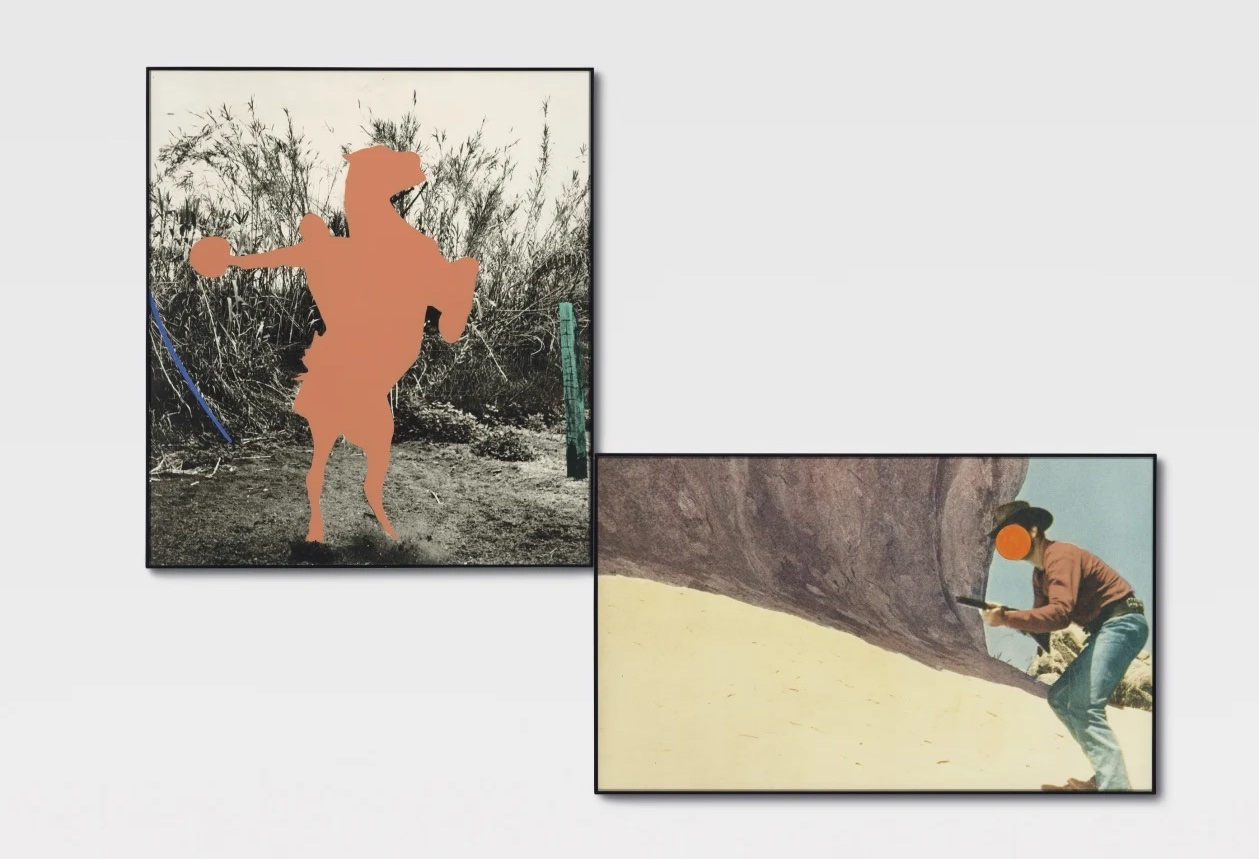
\includegraphics[width=\textwidth]{pulpogallery-john-baldessari-equestrian-flesh-1992.jpg}
    \caption{John Baldessari, \textit{Equestrian (Flesh) in Brackets with Orange Showdown}, 1992.}
    \label{fig:baldessari_equestrian}
\end{figure}


La obra \textit{Equestrian (Flesh) in Brackets with Orange Showdown} de John Baldessari ejemplifica el uso de la imagen-archivo como estrategia de producción artística\footnote{En el libro \textit{Arte y archivo, 1920-2010. Genealogías, tipologías y discontinuidades de Anna María Guasch} la autora dedica tudo un acápite titulado \textit{John Baldessari: el archivo como montaje} a explicar el  particular método de construcción de sentido visual empleado por Bassari mediante el montaje y decomposición lineal.}. Esta práctica, característica de su enfoque conceptual, se fundamenta en la apropiación y recontextualización de material visual preexistente. El artista no genera las fotografías originales, sino que las selecciona meticulosamente de archivos contemporáneos, incluyendo fotogramas cinematográficos hollywoodenses y otros materiales visuales de la cultura popular. Mediante intervenciones con pintura acrílica, Baldessari transforma el significado original de estas imágenes, generando nuevas capas de sentido que exploran cuestiones fundamentales sobre identidad, percepción y narrativa visual.

\begin{quote}
    El interés de Baldessari no se dirige, pues, a la historia en sí misma, sino a <<cómo contar la historia>> a través de la selección y combinación de imágenes. Al eliminar la narración lineal, deja que las diferencias de los elementos operen como un nudo de vías de comunicación a través del cual se posibilita un orden variable. Es precisamente la disposición sincrónica de las imágenes lo que permite que estas puedan finalmente ser leídas y releídas según múltiples direcciones.\parencite[p. 113-114]{Guasch2011}
\end{quote}

Estos "desechos" representan cristalizaciones modestas de la existencia, impurezas que se filtran entre las grietas y recovecos del fenómeno observado. En estas impurezas persiste el pasado, permitiéndonos manipular los hilos del tiempo y construir nuevas narrativas históricas.

 
\begin{figure}[h]
    \centering
    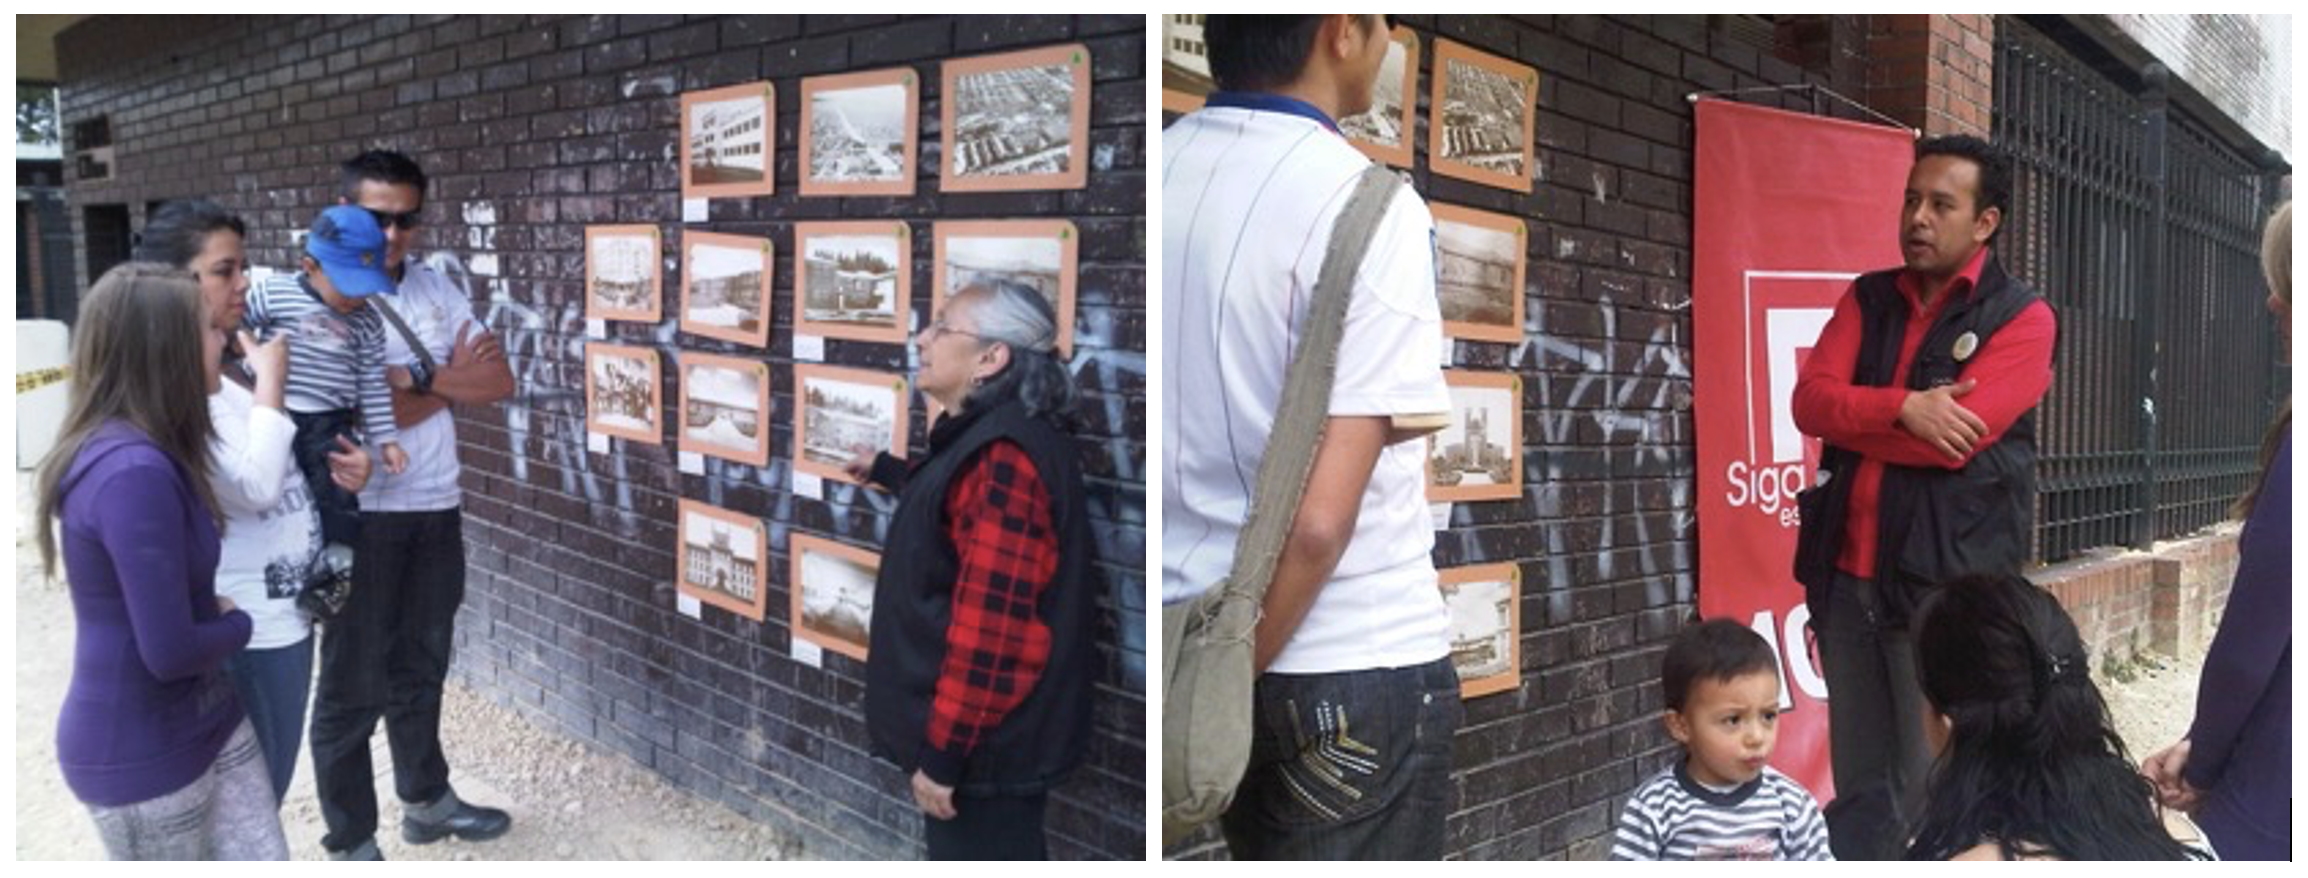
\includegraphics[width=\textwidth]{siga-esta-es-su-casa.png}
    \caption{Estación recorrido ``Siga esta es su casa'' (2008). Foto Archivo Margarita Castro}
    \end{figure}
    
La práctica de comprender el caso del Hospital San Juan de Dios a través de imágenes se estableció mucho antes que las experiencias de la mirada artística. En la Figura 1 se observan dos momentos de la visita "Siga esta es su casa", una de las estaciones de estos recorridos que originalmente se realizaban de forma autónoma como resistencia al olvido \parencite{Gongora2013}. Estos recorridos, inicialmente prohibidos durante el proceso de liquidación de la entidad, han resurgido después de muchos años. Sus promotores principales, la enfermera Margarita Castro y el arquitecto David Cristancho, son memoria viva que al guiar estos recorridos por el complejo hospitalario lo "actúan", manteniendo la estructura original. Durante 2022, esta práctica se transformó en una puesta en escena, desarrollándose en paralelo a otras acciones performativas y memoriales, como parte de un esfuerzo conjunto entre el Ministerio de Cultura, la Gobernación de Cundinamarca, el Instituto Distrital de Patrimonio Cultural (IDPC) y la Secretaría Distrital de Salud, para la intervención integral de siete de los diecisiete edificios de mayor valor patrimonial del Complejo Hospitalario \parencite{IDPCSanJuanDeDios}.
    
\begin{figure}[h]
    \centering
    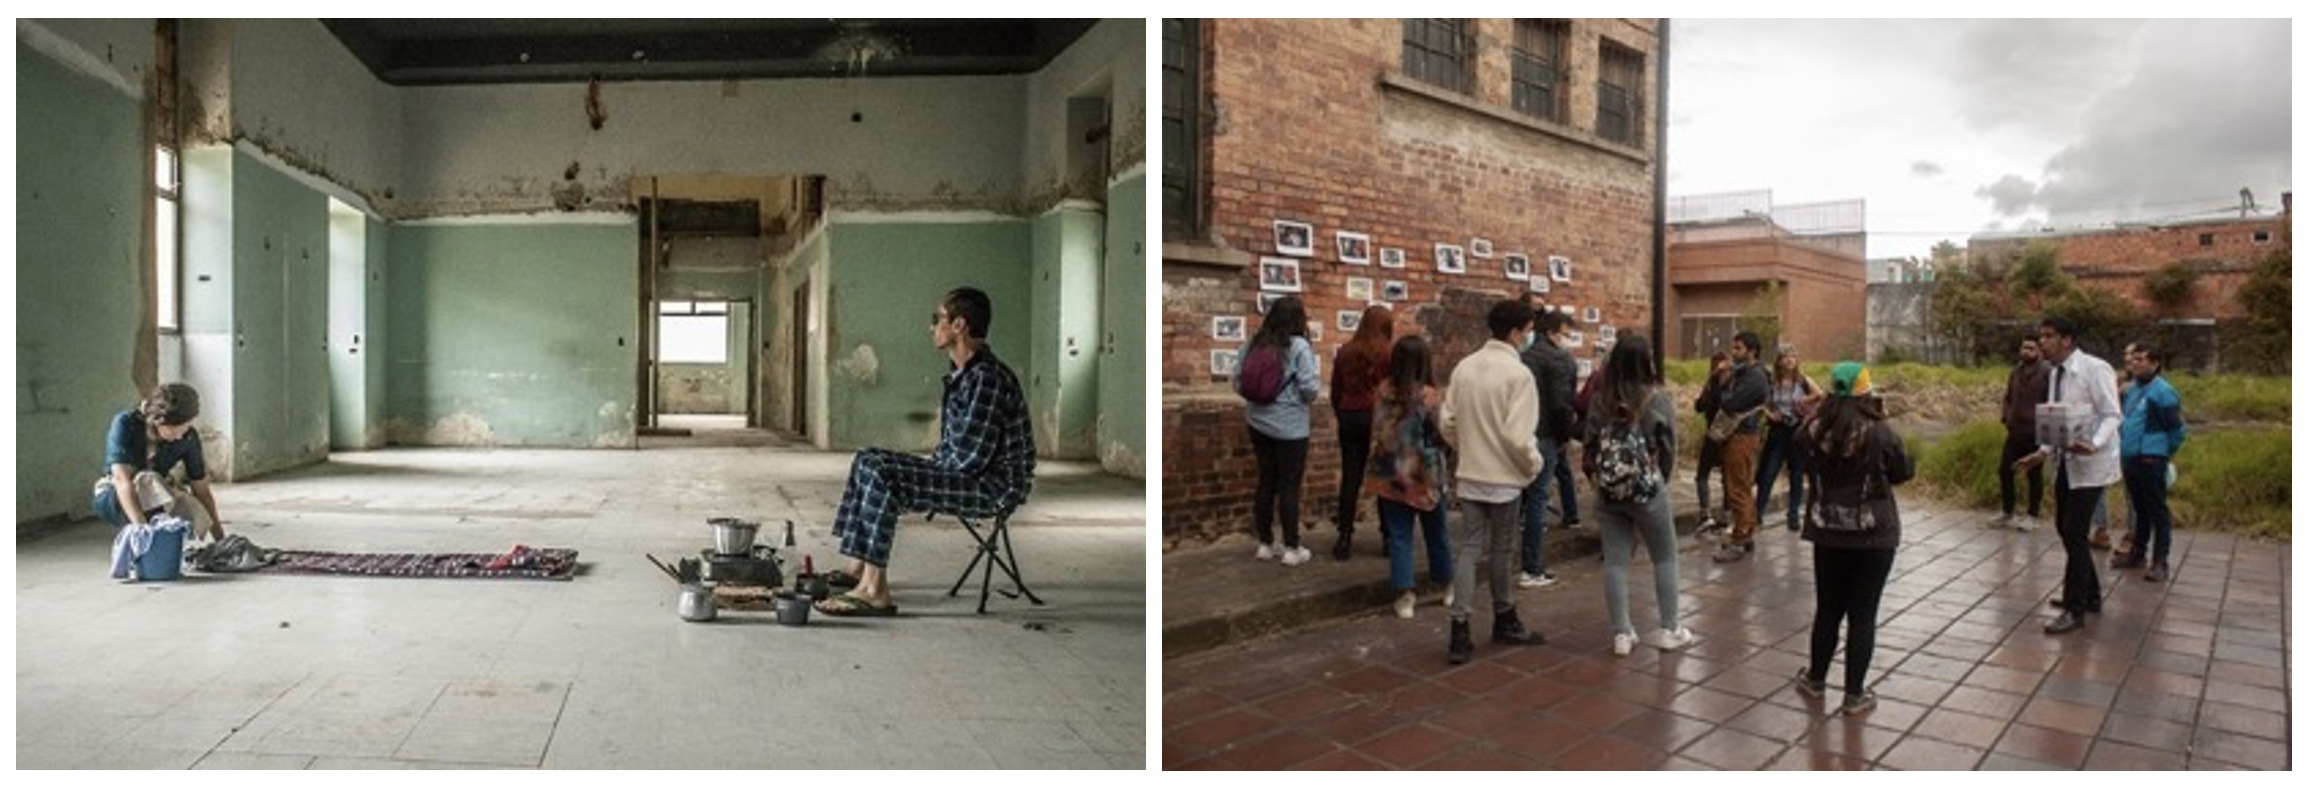
\includegraphics[width=\textwidth]{recorridos-idpc.png}
    \caption{Recorridos patrimoniales IDPC (2022). Foto: Juan Carlos Arroyo.}
\end{figure}

La Figura 3.3 muestra dos momentos de los recorridos patrimoniales coordinados por el IDPC. Estas prácticas performativas de sensibilización \parencite{Guasch2011} incluían la ilustración de momentos históricos mediante imágenes montadas sobre los muros exteriores del hospital. Cada imagen, impresa sobre papel, llevaba pequeñas notas históricas, replicando el formato de los recorridos originales del "Siga esta es su casa" realizados más de una década antes.

Resulta notable la capacidad del complejo hospitalario para convocar distintos actos de ver \parencite{Abril2007}, ya sean ejercicios de resistencia social, prácticas de memoria, acciones patrimoniales o, como ha ocurrido en varias ocasiones, escenario para la exhibición de obras de arte, relacionadas o no con el fenómeno de crisis del HSJD.

\begin{figure}[h]
    \centering
    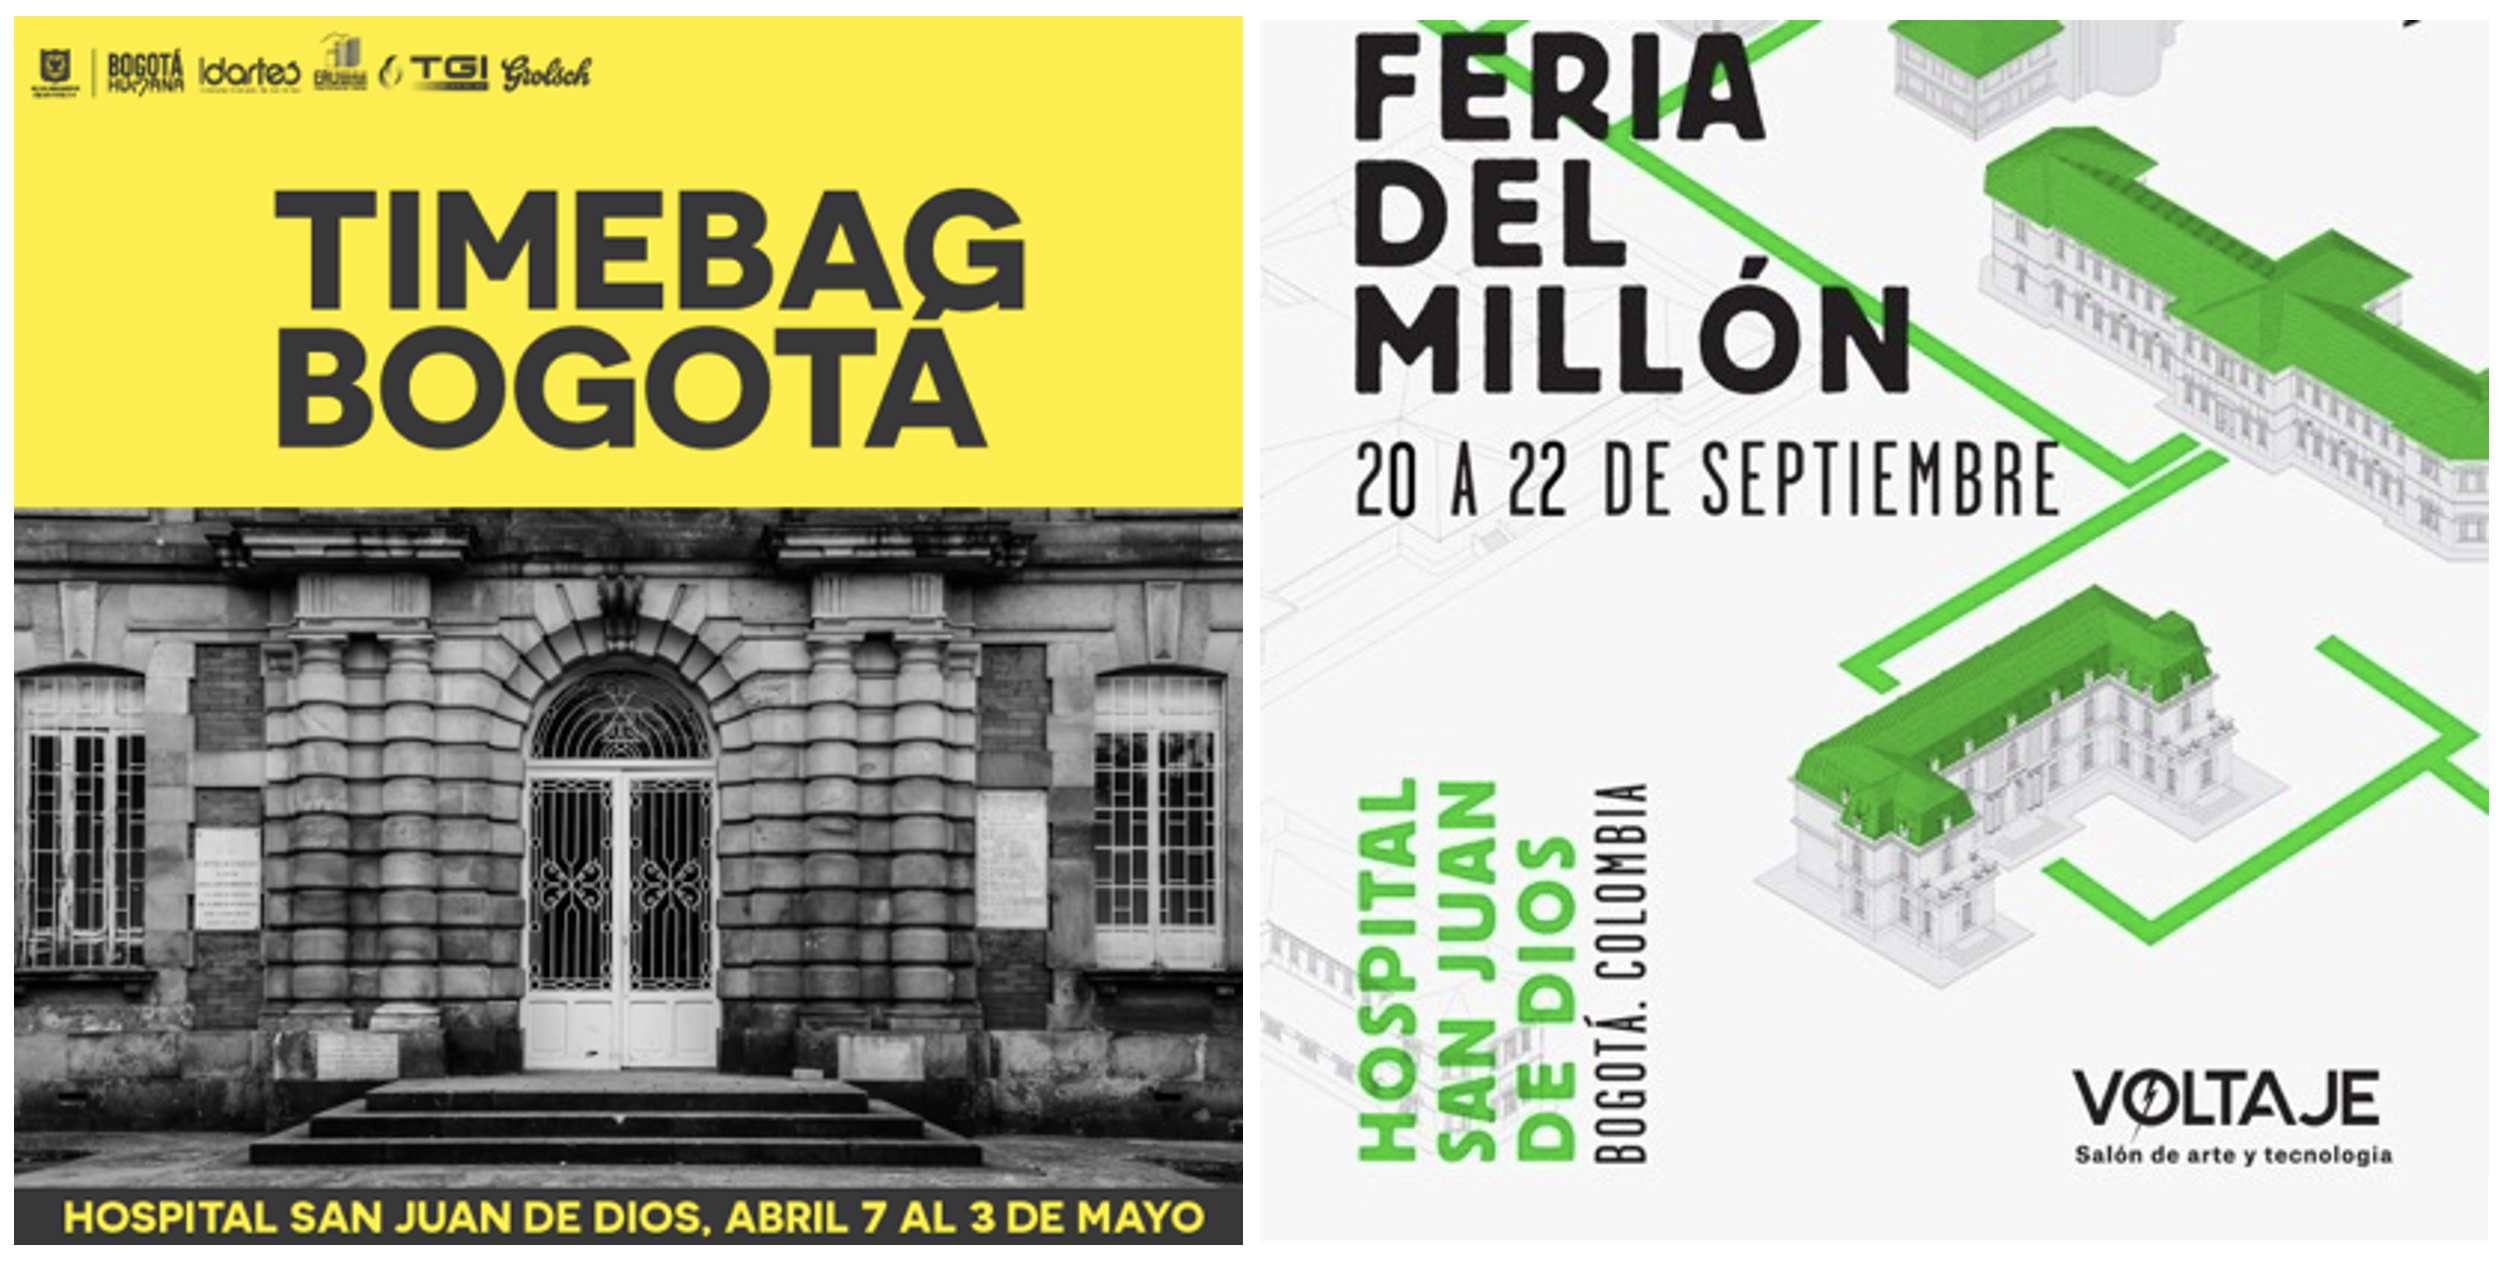
\includegraphics[width=\textwidth]{carteles.png}
    \caption{Carteles publicitarios TimeBag y Feria del Millón.}
\end{figure}

Dos eventos significativos fueron \textit{TimeBag Bogotá} y \textit{La Feria del Millón}, donde se evidenció la similitud en la práctica del montaje que, independiente de su intención, replica la práctica expositiva inherente al HSJD. Estos eventos crearon espacios de enunciación discursiva no-textual que, por desarrollarse dentro de este poderoso escenario patrimonial y simbólico, contribuyeron durante su efímera existencia al imaginario social sobre la crisis del San Juan.

El Hospital San Juan de Dios ha servido como escenario de montaje para prácticas memoriales, artísticas y performativas que, independientemente de su sensibilidad frente al fenómeno de crisis, generan imágenes de registro que se integran a la red significante e imaginaria, dada su escenificación reconocible al interior del complejo arquitectónico \parencite{BuckMorss1989}.

\begin{figure}[h]
    \includegraphics[width=\textwidth]{Pabellón San Lucas.png}
    \caption{Pabellón San Lucas (2001 y 2019). Archivo: IDPC.}
\end{figure}



\subsection*{El montaje}

La selección de imágenes constituye el primer paso fundamental en la construcción de sentido. Este proceso selectivo nos permite explorar la memoria social y nuestro inconsciente, revelando aspectos que normalmente permanecen ocultos tras la aparente cotidianidad de las imágenes.

El corpus de análisis, abordado mediante el método del montaje, comprende una colección de registros de obras de arte y activaciones culturales y memoriales realizadas en el Hospital San Juan de Dios (HSJD) entre 2000 y 2015. Adicionalmente, se incluyen imágenes significativas del año 2022 relacionadas con nuevas activaciones en torno al patrimonio.

Esta colección resulta particularmente reveladora por presentar imágenes que trascienden la cotidianidad operativa de un hospital. No se trata de reportería gráfica ni de imágenes inocentes; los registros artísticos y culturales materializan visualmente el San Juan como imágenes dialécticas, cargadas de deseos y potencial imaginativo. Como señala \parencite{DidiHuberman2011}: "Las imágenes dialécticas son símbolos de deseo (Wunsche). En ellas se presentan, al mismo tiempo que la cosa misma, el origen (Ursprung) y la decadencia (Untergang) de éste" (p. 169).

Durante el período activo de producción visual sobre el HSJD convergieron diversos intereses y formas de participación: artísticas, filosóficas, historicistas, antropológicas, de gestión cultural y agenciamiento social, memorial y comunitario.

Los registros visuales de estas intervenciones -sean obras plásticas, documentales, fotografías, dramaturgias o performances- han generado un repertorio de «memoria visual» que, en conjunto, enriquece la interpretación del fenómeno. Como señala \parencite{Abril2007}, esta construcción de sentido puede prescindir de la mediación textual o el ordenamiento cronológico, permitiendo que emerja la categoría benjaminiana de «imagen dialéctica», donde pasado y presente "destellan en una constelación" (p. 109).

La selección no pretende representar cronológicamente acontecimientos relevantes del HSJD, sino reunir diversas manifestaciones discursivas de resistencia sobre su crisis y cierre. Busca comprender tanto la emergencia de estas imágenes como sus contenidos en relación con el entorno vital y cultural de la crisis institucional.

El corpus de estudio comprende registros de obras plásticas, audiovisuales, fotográficas e instalaciones, junto con imágenes de archivos personales de los entrevistados. Estos objetos visuales serán "montados" en escenas para construir sentido mediante imágenes-síntoma y anacronismos.

Los criterios de selección se fundamentan en la presencia de atributos iconológicos, iconográficos, imágenes-síntoma y anacronismos. El montaje explora diversas conexiones entre acontecimientos, nociones y significaciones.

Como señala \parencite{Benjamin2004}, el montaje interrumpe el contexto establecido, forzando tanto al espectador como al actor a tomar postura ante los sucesos presentados. Esta interrupción no busca estimular, sino organizar la experiencia visual (p. 52).

Las obras artísticas, archivos fotográficos y dramatúrgicos seleccionados funcionan como memoria social, escenificando acontecimientos históricos y sociales que aluden a relaciones complejas, sin necesidad de responder a jerarquías, sistemas lógicos o narrativas lineales.

La metodología de análisis de imagen se fundamenta en dos marcos de referencia principales: el método de montaje propuesto por Walter Benjamin \parencite{BuckMorss1989} y el M12 desarrollado por Rubén Dittus \parencite{Aliaga2022}. Este proceso metodológico se estructura en dos fases, así:

\section{Selección}

a) \textbf{Elección de las imágenes:} La selección del corpus discursivo se constituye a partir de imágenes artísticas que abordan o se contextualizan en la crisis del Hospital San Juan de Dios de Bogotá. Este proceso implica una cuidadosa identificación y catalogación de obras que documentan visualmente este período histórico.

b) \textbf{Caracterización de manifestaciones del discurso:} El análisis comprende textos visuales que evidencian una corporeidad inequívoca del objeto de estudio. Este corpus integra registros de obras artísticas, material fotográfico y literatura generadora de imágenes mentales, todos ellos vinculados explícitamente con el fenómeno de crisis y cierre del Hospital San Juan de Dios. La selección prioriza aquellas manifestaciones que aportan significativamente a la construcción de la memoria colectiva del hospital.

c) \textbf{Descripción de la estructura:} El análisis de la estructura dialógica en los textos visuales seleccionados requiere la identificación sistemática de escenas que agrupan símbolos, signos denotativos, anacronismos e imágenes-síntoma. Este proceso analítico se fundamenta en los conceptos de la antropología de las imágenes y la sociosemiótica \parencite{Abril2007}, permitiendo una comprensión profunda de las capas de significado presentes en cada representación visual.

\section{Montaje}

a) \textbf{Escenarios para imaginarios:} El proceso interpretativo emerge desde la perspectiva del intérprete-espectador, estableciendo un diálogo dinámico entre la mirada y la imagen. El imaginario social que sustenta este dialogismo se fundamenta en la cultura visual contemporánea y la concepción colectiva del hospital: su pasado, su ideal y las transformaciones del imaginario social del HSJD provocadas por la crisis y el cierre \parencite{Gongora2013}. Esta aproximación permite comprender cómo las representaciones visuales contribuyen a la construcción de la memoria colectiva.

b) \textbf{Red significante:} El discurso seleccionado se articula en torno a conceptos totalizadores fundamentales: la salud pública, el cuidado humano y el imaginario del HSJD ideal. La crisis y el posterior cierre evidencian desequilibrios críticos en la operatividad hospitalaria, afectando no solo la prestación general de servicios de salud pública, sino también el cuidado humano, las historias de vida y la preservación de sujetos históricos y patrimoniales. Esta red de significados permite comprender la complejidad del impacto social y cultural de la crisis hospitalaria.


\phantomsection
\printbibliography
\addcontentsline{toc}{chapter}{Bibliografía}

\end{document}